%\documentclass{article}


\documentclass[a4paper,11pt]{article}
\pdfoutput=1 % if your are submitting a pdflatex (i.e. if you have
             % images in pdf, png or jpg format)

\usepackage{jheppub} % for details on the use of the package, please
                     % see the JHEP-author-manual




%\usepackage[utf8]{inputenc}
\usepackage[T1]{fontenc}
%\usepackage{geometry}
%\geometry{a4paper}
\usepackage{hyperref}
\usepackage{graphicx}
\usepackage[table]{xcolor}
\usepackage{graphicx}
\usepackage{url}
\usepackage{hyperref}
\usepackage{enumitem}
\usepackage{booktabs}
\usepackage{rotating}
\usepackage[frenchb]{babel}


\definecolor{light-gray}{gray}{0.95}
\newcommand{\code}[1]{\colorbox{light-gray}{\texttt{#1}}}
\newcommand{\codewhite}[1]{\colorbox{white}{\texttt{#1}}}


\title{Machine Learning Applied to Cancer Survival Prognosis}
\author{Innovative Oncology Business Solutions \\
 4901 Lang Ave NE, Ste 204 \\
Albuquerque, NM 87109 \\
\url{http://www.innovativeobs.com/contact/}}
\date{}



\abstract{This short note describes activties at 
\href{http://www.innovativeobs.com/}{IOBS} using two state-of-the-art machine learning techniques (random forests and neural networks) 
that leverage the publically available information in the Surveillance, Epidemiolgy, and End Results (SEER) Program database of the National Cancer Institute (NCI) to make highly accurate predictive models of cancer survival curves. The most recent application of these types of models to prostate cancer also includes the effect of radiation therapy on survival prognosis. These techniques can easily be modified and applied to similar problem sets facing 
Ion Beam Applications SA, such as providing a rigorous robust model to ascertain the Cancer Survival prognosis associated with the use of Proton Therapy to help measure the value proposition of outcomes to cost.}


\begin{document}
\maketitle
\flushbottom
%\tableofcontents


\section{Introduction and Background}
\label{sec:intro}



Extracting actionable information from data is changing the fabric of modern business. A class of techniques that transforms data into actionable information goes by the name of Machine Learning \cite{pythonmachinelearning}.
Machine Learning has recently become a popular method to answer questions and solve problems that are too complex to solve via traditional methods, such as that of accurately predicting cancer survival prognosis curves for individual patients.
The Surveillance, Epidemiolgy, and End Results (SEER) Program of the National Cancer Institute (NCI) has been collecting data because intuitively researchers feel confident that this data is capturing information that has buried within it useful information in the form of  relationships between the types of data collected (demographic as well as staging information) and the survival outcomes.
Though this relationship evades capture by traditional methods, it is possible to surface it with the two machine learning techniques known as \textbf{Random Forests} and \textbf{Neural Networks}. These two methods produce very similar results when applied to the SEER dataset, and are based on two almost diametrically opposed learning philosophies, which lends confidence in the validity of the results.

The Surveillance, Epidemiolgy, and End Results (SEER) Program of the National Cancer Institute (NCI) is the most recognized authoritative source of information on cancer incidence and survival in the United States. SEER currently collects and publishes cancer incidence and survival data from population-based cancer registries covering approximately 28 percent of the US population.


Quoting directly from the SEER
website \citep{seerwebsite}:

\begin{quote}
The SEER program registries routinely collect data on patient demographics, primary tumor site, tumor morphology and stage at diagnosis, first course of treatment, and follow-up for vital status. This program is the only comprehensive source of population-based information in the United States that includes stage of cancer at the time of diagnosis and patient survival data. The mortality data reported by SEER are provided by the National Center for Health Statistics. The population data used in calculating cancer rates is obtained periodically from the Census Bureau. Updated annually and provided as a public service in print and electronic formats, SEER data are used by thousands of researchers, clinicians, public health officials, legislators, policymakers, community groups, and the public.
\end{quote}


One characterstic of the SEER data and that is shared by many datasets in the medical field 
goes by the name of "censored data.'' The SEER data contains the number of months each patient survived, as well as an indicator variable showing whether or not the patient is still alive at the end of the data collection period.
Methods to deal effectively with this kind of "right-censored data'' include Kaplan-Meier curves
and Cox's Proportional Hazard models \cite{cam}. The Kaplan-Meier techniques only give estimates for cohorts of patients and are not applicable for predicting the surival curve for a single patient, and the Cox Proportional Hazard models require a fairly restrictive set ot assumptions to be satisifed in order to yield reliable results. In addition, the Cox Proportional Hazard models are not able to capture the nonlinear relationships between the given data fields that go into making predictions; they can only capture the first-order linear relationships.

Previous work by other researchers in the community applying machine learning methods to subsets of the SEER data include creative attempts to deal with the problems presented by  "right-censored data." The authors of ~\cite{ISI:000337467400005} use semi-supervised learning techniques to predict 5 year survival, essentially imputing values for SEER records where the survival months infomation is censored at a value less than 5 years. The authors of ~\cite{ISI:000355882700012} investigate the effects of comordbidities; i.e., patients with two different cancer diagnosises, but their treatment of the censored data underestimates the survival probabilities. All records representing patients who survived at least 60 months as well as all those who died earlier than 60 months were considered, but patients alive prior to 60 months but censored out of the study before 60 months were not included. This treatment biases the data and the predictions, leading to overly pessimistic survival probablilites predicted by the trained models.



To overcome these limitations of the traditional methods, IOBS has applied a little-known technique not seen in the literature to transform the SEER data to make it amenable to more powerful machine learning methods. The essential idea is to recast the problem to an appropriate discrete classification problem instead of a regression problem (predicting survival months). Treating months after diagnosis as just another discrete feature, the SEER data (or any other right-censored data) can be transformed simply so as to make predictions for the hazard function
 (the probability of dying in the next month, given that the patient has not yet died).
The full survival function can then be derived from the hazard function.
Details of this transformation can be found in this blog post \cite{kuhn}, and pseudocode for this transformation is provided in section~(\ref{subsec:pseudocode}).






%%%%%%%%%%%%%%%%%%%%%%%%%%%%%%%%%%%%%%%%
%\section{Introduction}

%This short note describes activties at 
%\href{http://www.innovativeobs.com/}{IOBS} using two state-of-the-art machine learning %techniques (random forests and neural networks) 
%that leverage the publically available information in the Surveillance, Epidemiolgy, and End %Results (SEER) Program database of the National Cancer Institute (NCI) to make highly %accurate predictive models of cancer survival curves. The most recent application of these %types of models to prostate cancer also includes the effect of radiation therapy on survival %prognosis. These techniques can easily be modified and applied to similar problem sets facing 
%Ion Beam Applications SA, such as providing a rigorous demonstration of the effecicacy of %proton therapy.



 



%\section{SEER Data}

%The Surveillance, Epidemiolgy, and End Results (SEER) Program of the National Cancer %Institute (NCI) is the most recognized authoritative source of information on cancer incidence %and survival in the United States. SEER currently collects and publishes cancer incidence and %survival data from population-based cancer registries covering approximately 28 percent of the %US population.

%Quoting directly from the SEER
%website:\footnote{National Cancer Institute, the Surveillance, Epidemiology, and End Results %Program. Available at: \url{http://seer.cancer.gov/about/}}

%\begin{quote}
%The SEER program registries routinely collect data on patient demographics, primary tumor %site, tumor morphology and stage at diagnosis, first course of treatment, and follow-up for vital %status. This program is the only comprehensive source of population-based information in the %United States that includes stage of cancer at the time of diagnosis and patient survival data. %The mortality data reported by SEER are provided by the National Center for Health Statistics. %The population data used in calculating cancer rates is obtained periodically from the Census %Bureau. Updated annually and provided as a public service in print and electronic formats, %SEER data are used by thousands of researchers, clinicians, public health officials, legislators, %policymakers, community groups, and the public.
%\end{quote}



%One characterstic of the SEER data and that is shared by many datasets in the medical field 
%goes by the name of ``censored data.`` The SEER data contains the number of months each %patient survived, as well as an indicator variable showing whether or not the patient is still %alive at the end of the data collection period. For example, some patients that were diagnosed %with colon cancer in June of 2010 and that are still alive at the end of the last SEER data %release, will have some value for survival months, say 60 months, as well as an indicator %variable, `vital$\_$status$\_$recode`, indicating that they are still alive. Other patients also %diagnosed in June of 2010 will have some value for surival months listed, say 17 months, and %for these patients then indicator variable `vital$\_$status$\_$recode` will indicate that they are %deceased. 
%Methods to deal effectively with this kind of `right-censored data` include Kaplan-Meier curves
%and Cox's Proportional Hazard models.\footnote{ Cam Davidson-Pilon, ``Quickstart -- lifelines %0.8.0.1 documentation,`` accessed 11 Jan 2016, \url{http://lifelines.readthedocs.org/en/latest/%Quickstart.html}.} The Kaplan-Meier techniques only give estimates for cohorts of patients and %are not applicable for predicting the surival curve for a single patient, and the Cox Proportional %Hazard models require a fairly restrictive set ot assumptions to be satisifed in order to yield %reliable results. In addition, the Cox Proportional Hazard models are not able to capture the %nonlinear relationships between the given data fields that go into making predicitons; they can %only capture the first-order linear relationships.

%To overcome these limitations of the traditional methods, IOBS has applied a little-known %technique to transform the SEER data to make it amenable to more powerful machine learning %methods. The basic idea is to explictly consider each month of survival after diagnosis as a new %data point. For example, a patient that is currenly listed in the SEER data with a `vital$\_%%$status$\_$recode` indicating that they are still alive, and with a `survival$\_$months` value of %5, would be handled by replacing this data record with 6 additional records corresponding to %this patient.
%These additional records are identical to the orginal, with the important exception of `survival$%\_$months` ranging from 0 through 5. Similar transformations can be applied to the data %records where the `vital$\_$status$\_$recode` variable indicates that the patient is deceased.
%A duplicate of the record is created for each month prior to the value of `survival$\_$months.`
%For example, if a patient is recorded as deceased and as having survived 10 months, the %transformed data set would contain 11 records for that patient, where `survival$\_$months` %ranges from 0 through 10, and `vital$\_$status$\_$recode` indicates that they are alive for %months 0 through 9, and deceased for month 10.
%Details of this transformation can be found in this blog post.\footnote{Ben Kuhn, ``Decision %trees for survival analysis,`` accessed 11 Jan 2016, \url{http://www.benkuhn.net/survival-%trees}.}







\section{Machine Learning Algorithms}


Extracting actionable information from data is changing the fabric of modern business. A class of techniques that performs this transformation of data into actionable information goes by the name of Machine Learning.
%Machine Learning has recently become a popular method to answer questions and solve %problems that are too complex to solve via traditional methods. 
%One class of problems for which these algorithms are approriate is generally referred to as 
%\textit{function approximation}. SEER has been collecting data because intuitively researchers %feel confident that this data is capturing information that has buried within it useful %information in the form of  relationships between the types of data collected (demographic as %well as staging information) and the survival outcomes.
Though these relationships often evades capture by traditional methods, it is possible to surface them with the two machine learning techniques known as \textbf{Random Forests} and \textbf{Neural Networks}.
These two methods produce very similar results when applied to the SEER dataset, and are based on two almost diametrically opposed learning philosophies, which lends confidence in the validity of the results. 
Random Forests are made up of an ensemble of independet \textbf{Decision trees} that are purposefully exposed to only subsets of the data. The general philosophy is that popularized by the book "The Wisdom of Crowds''~\cite{wisdom}.
The idea is that a large number of independent not necessarily expert opinions converge on the correct answer when averaged. The success of this philosophy of prediction was startingly shown by the success of the political and world event predictions made by the prediction market site Intrade, before its forced closure by the Commodity Futures Trading Commission~\cite{cassidy}. %\footnote{``What killed Intrade?``, John Cassidy, \textit{The New Yorker}, 10 Mar, 2013, %accessed 11 Jan 2016, \url{http://www.newyorker.com/news/john-cassidy/what-killed-%intrade}.} 
 The other method used by IOBS to develop predictive models are called neural networks, and are modelled on how the human brain learns high level concepts from lower level ones. The philosophy behind the training and achieved accuracies of neural network classifiers and predictors is that of going to a seasoned expert. A Neural network trains from repeated exposure to the training data and improves its predictions with each pass over the data. The general philosophy is simlar to that represented by the well-known maxim that it takes 10,000 hours to become an `expert` in any given field~\cite{outliers}.
%\footnote{``The 10,000 Hour Rule,` Malcolm Gladwell, accessed 11 Jan 2016, \url{http://%gladwell.com/outliers/the-10000-hour-rule/}.}





\subsection{Decision Trees and Random Forests}

\textbf{Decision tree} classifiers are attractive models if we care about interpretability. Like the name decision tree suggests, we can think of this model as breaking down our data by making decisions based on asking a series of questions.
Based on the features in our training set, the decision tree model learns a series of questions to infer the class labels of the samples. 
%This procedure works with both categorical variables %and real numbers as features. For example, we could simply define a cut-off value along the %sepal width feature axis and ask a binary question "sepal width " $\geq$ 2.8 cm?"
%Using the decision algorithm, we start at the tree root and split the data on the feature that %results in the largest information gain (IG), which will be explained in more detail in the %following section. In an iterative process, we can then repeat this splitting procedure at each %child node until the leaves are pure. This means that the samples at each node all belong to %the same class. In practice, this can result in a very deep tree with many nodes, which can %easily lead to overfitting. Thus, we typically want to prune the tree by setting a limit for the %maximal depth of the tree.

%Decision trees are very simple yet powerful supervised learning methods, which construct a %yield a decision tree model that can be used to make predictions.
%Binary decision trees operate by subjecting attributes to a series of binary (yes/no) decisions. %Each decision leads to one of two possibilities. Each decision leads to another decision or it %leads to prediction. An example of a trained tree will help cement the idea.
%Decision trees are tree-like graphs that model a decision. They are analogous to the parlor %game Twenty Questions. In Twenty Questions, one player, called the answerer, chooses an %object but does not reveal the object to the other players, who are called questioners. The %object should be a common noun, such as "guitar" or "sandwich", but not "1969 Gibson Les %Paul Custom" or "North Carolina". The questioners must guess the object by asking as many as %twenty questions that can be answered with yes, no, or maybe. An intuitive strategy for %questioners is to ask questions of increasing specificity; asking "is it a musical instrument?" as %the first question will not efficiently reduce the number of possibilities. The branches of a %decision tree specify the shortest sequences of explanatory variables that can be examined in %order to estimate the value of a response variable.

%In order to split the nodes at the most informative features, we need to define an objective %function that we want to optimize via the tree learning algorithm. Here, our objective function %is to maximize the information gain at each split, which we define as follows:


%\begin{equation}
%IG(D_{p},f) = I(D_{p}) - \sum_{j=1}^{m} \frac{N_{j}}{N_{p}} I(D_{j})
%\end{equation}


%Here, $f$ is the feature to perform the split, $D_{p}$ and $D_{j}$ are the dataset of the %parent and 
%$j^{th}$ child node, $I$ is our impurity measure, $N_{p}$ is the total number of samples at %the 
%parent node, and $N_{j}$ is the number of samples in the $j^{th}$ child node.

%As we can see, the information gain is simply the difference between the impurity of the %parent node and the sum of the child node impurities - the lower the impurity of the child %nodes, the larger the information gain. However, for simplicity and to reduce the combinatorial %search space, most libraries 
%(including scikit-learn) implement binary decision trees. This means that each parent node is %split into two child nodes, $D_{left}$ and $D_{right}$:

%\begin{equation}
%IG(D_{p}, a) = I(D_{p}) - \frac{N_{left}}{N_{p}} I(D_{left}) - \frac{N_{right}}{N_{p}} %I(D_{right})
%\end{equation}

%Now, the three impurity measures or splitting criteria that are commonly used in binary %decision trees are \textbf{Gini impurity} ($I_{G}$), \textbf{entropy} ($I_{H}$), and the
%\textbf{classification error} ($I_{E}$).

%Let's start with the definition of entropy for all \textbf{non-empty} classes $p(i | t) \neq 0$:

%\begin{equation}
%I_{H}(t) = -\sum_{i=1}^{c} p(i | t) \log_{2}{p(i|t)}
%\end{equation}


%Here, $p(i | t)$ is the proportion of the samples that belong to class c for a particular node $t$.
%The entropy is therefore 0 if all samples at a node belong to the same class, and the entropy is %maximal if we have a uniform class distribution. For example, in a binary class setting, the 
%entropy is 0 if $p(i=1|t) = 1$ or $p(i=0|t) = 0$. If the classes are distributed uniformly with 
%$p(i=1|t) = 0.5$ and $p(i=0|t) = 0.5$, the entropy is 1. Therefore, we can say that the entropy %criterion attemps to maximize the mutual information in the tree.

%Intuitively, the Gini impurity can be understood as a criterion to minimize the probability of %misclassification:

%\begin{equation}
%I_{G}(t) = \sum_{i=1}^{c}p(i | t) ( 1 - p(i|t)) = 1 - \sum_{i=1}^{c} p(i | t)^{2}
%\end{equation}



%Similar to entropy, the Gini impurity is maximal if the classes are perfectly mixed, for example, %in a binary class setting $(c = 2)$:

%\begin{equation}
%1 - \frac{1}{2}^{2} - \frac{1}{2}^{2} = 1 - \frac{1}{4} - \frac{1}{4} = \frac{1}{2}
%\end{equation}


%However, in practice both the Gini impurity and entropy typically yield very similar results and %it is often not worth spending much time on evaluating trees using different impurity criteria %rather than experimenting with different pruning cut-offs.

%Another impurity measure is the classification error:

%\begin{equation}
%I_{E} = 1 - \mbox{max}\{ p(i|t) \}
%\end{equation}


%We can illustrate these concepts by looking at the two possible splitting scenarios shown 
%in Figure \ref{fig:split}.



%\begin{figure}[!ht]
% \caption{Example decision tree splitting.}
%  \label{fig:split}
%  \centering
%    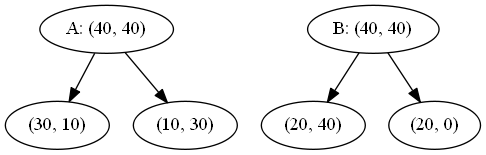
\includegraphics[scale=0.5]{mdga}
%\end{figure}


%We start with a dataset $D_{p}$ at the parent node $D_{p}$ that consists of 40 samples from %class 1 
%and 40 samples from class 2 that we split into two datasets $D_{left}$ and $D_{right}$, %respectively.
%The information gain using the classificaiton error as a splitting condition would be the same
%$(IG_{E} = 0.25)$ in both scenario A and B:


%\begin{eqnarray}
%I_{E}(D_{p})  & = & 1 - 0.5  =   0.5  \\
%\mbox{A} :I_{E}(D_{left}) & =  & 1 - \frac{3}{4}  =   0.25 \\
%\mbox{A} :I_{E}(D_{right}) & = & 1 - \frac{3}{4}   =  0.25 \\
%\mbox{A} :IG_{E} & = & 0.5 - \frac{40}{80}\frac{1}{4} - \frac{40}{80}\frac{1}{4}   =  
%\frac{1}{4} \\
%\mbox{B} :I_{E}(D_{left}) & = & 1 - \frac{4}{6} =  \frac{1}{3} \\
%\mbox{B}:I_{E}(D_{right}) & = & 1 - \frac{1}{1}  =   0 \\
%\mbox{B}:IG_{E} & = & 0.5 - \frac{6}{8} \frac{1}{3} - \frac{2}{8} \times  0  =  \frac{1}{4} 
%\end{eqnarray}


%However, the Gini impurity would favor the split in scenario $B$ $(IG_{G} = 0.1\bar{6})$ over
%scenario $A$ $(IG_{G} = 0.125)$, which is indeed more pure:


%\begin{eqnarray}
%I_{G}(D_{p}) & = & 1 - \frac{1}{2}^{2} - \frac{1}{2}^{2} = \frac{1}{2} \\
%\mbox{A}:I_{G}(D_{left}) &  = & 1  - \frac{3}{4}^{2} - \frac{1}{4}^{2} = \frac{3}{8} \\
%\mbox{A}:I_{G}(D_{right}) & = &  1 - \frac{1}{4}^{2} - \frac{3}{4}^{2} = \frac{3}{8} \\
%\mbox{A}:IG_{G}  & = & \frac{1}{2} - \frac{40}{80}\frac{3}{8} - \frac{40}{80}\frac{3}{8} = %\frac{1}{8} \\
%\mbox{B}:I_{G}(D_{left})  & = & 1 - \frac{2}{6}^{2} - \frac{4}{6}^{2} = \frac{4}{9} \\
%\mbox{B}:I_{G}(D_{right})  & = & 1 - \frac{20}{20}^{2} = 0 \\
%\mbox{B}:IG_{G} & = &  \frac{1}{2} - \frac{60}{80}\frac{4}{9} = \frac{1}{2} - \frac{1}{3} = %\frac{1}{6}
%\end{eqnarray}



%Decision trees can build complex decision boundaries by dividing the feature space into %rectangles. 
%Figure \ref{fig:rectangles} shows an example for the famous Iris dataset using only two %features.
%However, we have to be careful since the deeper the decision tree, the more complex the %decision bounday becomes, which can easily result in overfitting.
% Using scikit-learn, we will now train a decision tree with a maximum depth of 3 using entropy %as a criterion for impurity. Although feature scaling may be desired for visualization purposes, %not that feature scaling is not a requirement for decision tree algorithms. 




%\begin{figure}[!ht]
% \caption{Example decision tree decision boundaries.}
% \label{fig:rectangles}
% \centering
%    \includegraphics[scale=0.8]{iris}
%\end{figure}



%Figure \ref{fig:questions} displays the questions inferred from growing the decision tree on %this dataset, where the questions are automatically generated from maximizing the information %gain.


%\begin{figure}[!ht]
% \caption{Explicit Decision Tree.}
%  \label{fig:questions}
%  \centering
%    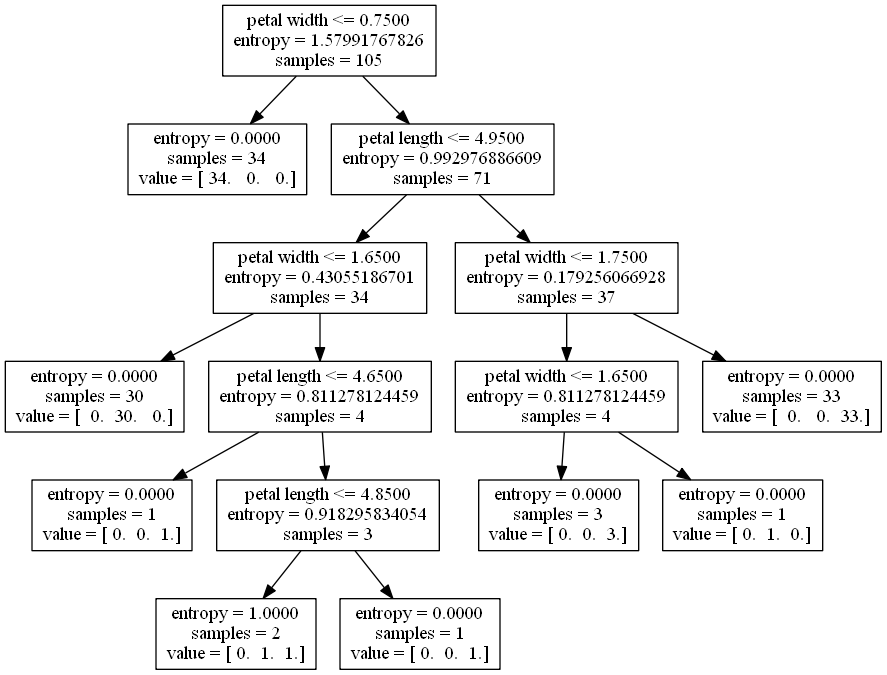
\includegraphics[scale=0.5]{questions}
%\end{figure}

%The random forests algorithm was developed by the late Berkeley professor Leo Breiman and %Adele Cutler. Random forests generates its sequence of models by training them on subsets of %the data. The subsets are drawn at random from the full training set. One way in which the %subset is selected is to randomly sample rows with replacement. The other random element is %that the training sets for the individual trees in the random forests ensemble don’t incorporate %all the attributes but take a random subset of the attributes also.


\textbf{Random forests} have gained huge popularity in applications of machine learning during the last decade due to their good classification performance, scalability, and ease of use. Intuitively, a random forest can be considered as an \textit{ensemble of decision trees}. The idea behind ensemble learning is to combine \textbf{weak learners} to build a more robust model, a \textbf{strong learner}, that has a better generalization error and is less susceptible to overfitting. 
%The random forest algorithm can be summarized in four simple steps:



%\begin{enumerate}
%\item Draw a random \textbf{bootstrap} sample of size \textit{n} (randomly choose \textit{n} %samples from the training set with replacement).
%\item Grow a decision tree from the bootstrap sample. At each node:
%   \begin{enumerate}
%    \item Randomly select d features without replacement.
%    \item Split the node using the feature that provides the best split according to the objective %function, for instance, by maximizing the information gain.
%    \end{enumerate}
%\item Repeat the steps 1 to 2 \textit{k} times.
%\item Aggregate the prediction by each tree to assign the class label by \textbf{majority vote}. 
%\end{enumerate}




%There is a slight modification in step 2 when we are training the individual decision trees: %instead of evaluating all features to determine the best split at each node, we only consider a %random subset of those.

%Although random forests don't offer the same level of interpretability as decision trees, a big %advantage of random forests is that we don't have to worry so much about choosing good %hyperparmeter values. We typically don't need to prune the random forest since the ensemble %model is quite robust to noise from the individual decision trees. The only parameter that we %really need to care about in practice is the number of trees $k$ (step 3) that we choose for the %random forest. Typically, the larger the number of trees, the better the performance of the %random forest classifier at the expense of an increased computational cost.

%Although it is less common in practice, other hyperparameters of the random forest classifier %that can be optimized are the size \textit{n} of the bootstrap sample (step 1) and the number %of features \textit{d} that are randomly chosen for each split (step 2.1), respectively. Via the %sample size \textit{n} of the bootstrap sample, we control the bias-variance tradeoff of the %random forest. By choosing a larger value for \textit{n}, we decrease the randomness and thus %the forest is more likely to overfit. On the other hand, we can reduce the degree of overfitting %by choosing smaller values for \textit{n} at the expense of the model performance. In most %implementations, including the `RandomForestClassifier` implementation in scikit-learn, the %sample size of the bootstrap sample is chosen to be equal to the number of samples in the %orginal training set, which usually provides a good bias-variance tradeoff. For the number of %features \textit{d} at each split, we want to choose a value that is smaller than the total %number of features in the training set. A reasonable default that is used in scikit-learn and %other implementations is 
%$d = \sqrt{m}$, where $m$ is the number of features in the training set.


The goal behind \textbf{ensemble methods} is to combine different classifiers into a meta-classifier that has a better generalization performance than each individual classifier alone. For example, assuming that we collected predictions from 10 experts, ensemble methods would allow us to strategically combine these predictions by the 10 experts to come up with a prediction that is more accurate and robust than the predictions by each individual expert.

%To illustrate why ensemble methods can work better than individual classifiers alone, let's apply %the simple concepts of combinatorics. For the following example, we make the assumption that %all \textit{n} base classifiers for a binary classification task have an equal error rate $\epsilon$. %Furthermore, we assume that the classifiers are independent and the error rates are not %correlated. Under these assumptions, we can simply express the error probability of an %ensemble of base classifiers as a probability mass function of a binomial distribution:

%\begin{equation}
%P (y \geq k) = \sum_{k}^{n} {n \choose k} \epsilon^{k} (1 - \epsilon)^{n - k} =   \epsilon_{ensemble}
%\end{equation}


%Here, ${n \choose k}$ is the binomial coefficient n choose k. In other words, we compute the %probability that the prediction of the ensemble is wrong. Now let's take a look at a more %concrete example of 11 base classifiers $(n = 11)$ with an error rate of 0.25 $(\epsilon = 0.25)%$:

%\begin{equation}
%P (y \geq k) = \sum_{k=6}^{11} {11 \choose k} 0.25^{k} (1 - 0.25)^{11 - k} = 0.034
%\end{equation}

Figure~(\ref{fig:ensemble}) illustrates the power of ensemble methods; the Figure illustrates how the ensemble error rate is much lower than the Base learner error rate, as long as the Base learner error rate is less than 0.5. The Figure illustrates this effect for an ensemble of 500 base learners.







%As we can see, the error rate of the ensemble (0.034) is much lower than the error rate of %each individual classifier (0.25) if all the assumptions are met. Note that, in this simplified %illustration, a 50-50 split by an even number of classifiers \textit{n} is treated as an error, %whereas this is only trye half of the time. To compare such an idealistic ensemble classifier to a %base classifier over a range of different base error rates, let's implement the probability mass %function in Python:

\begin{figure}[!ht]
  \centering
    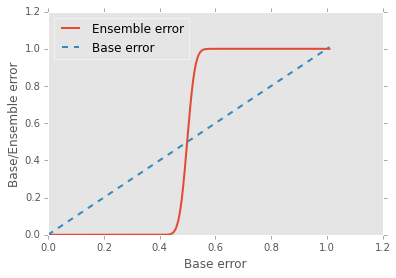
\includegraphics[scale=1.0]{ensemble}
\caption{\label{fig:ensemble} Illustration of ensemble methods showing how a collection of base learners with poor accuracy can combine to produce an accurate ensemble learner.}
\end{figure}


IOBS has chosen to use the Python scikit-learn implemenation of the Random Forest machine learning classifier~\cite{rf}.
Random Forests are frequent winners of the Kaggle machine learning competitions~\cite{kagglerf}.




\subsection{Neural Networks and Deep Learning}

Neural networks are a biologically-inspired progrmming paradigm that enable computers to learn from observational data~\cite{deeplearning}.
%As you may know, \textbf{deep learning} is getting a lot of press and is without any doubt the %hottest topic in the machine learning field.
Deep learning can be understood as a set of algorithms that were developed to train \textbf{artificial neural networks} with many layers most efficiently.
 Neural networks are a hot topic not only in academic research, but also in big technology companies such as Facebook, Microsoft, and Google who invest heavily in artificial neural networks and deep learning research. As of today, complex neural networks powered by deep learning algorithms are considered as state-of-the-art when it comes to complex problem solving such as image and voice recognition.
In addition, the pharmaceutical industry recently started to use deep learning techniques for drug discovery and toxicity prediction, and research has shown that these novel techniques substantially exceed the performance of traditional methods for virtual screening~\cite{toxicity}.

IOBS has chosen to use the neural network implementation Keras developed at MIT.
Keras was initially developed as part of the research effort of project ONEIROS (Open-ended Neuro-Electronic Intelligent Robot Operating System)~\cite{keras}.
Keras is a minimalist, highly modular neural networks library, written in Python and capable of running on top of either TensorFlow or Theano.

\section{Survival Curve Prediction Apps}

Below is a list of some web applications developed by IOBS.
For each of the cancer types (colon, breast, lung, and prostate), a model has been developed using random forests and one using neural networks. The models were evaluted using the AUC (Area Under Curve) performance evaluation metric on test data (data not used in the training of the models), typically achieving AUC scores  $\approx .8$, as shown in Table~(\ref{tab:AUC}).\footnote{``AUC | Kaggle,'' Kaggle Website, \url{https://www.kaggle.com/wiki/AUC}, accessed 11 Jan 2016.}
 

\begin{table}[tbp]
\begin{center}
\rowcolors{1}{white}{light-gray}
\begin{tabular}{lrrr}
\toprule
%\rowcolors{1}{white}{yellow}
%\hline
Model & 6 Months AUC & 12 Months AUC & 60 Months AUC \\ 
\midrule
Breast RF &  .846       &     .885           &  .844 \\ 
Breast NN &   .855      &     .867      &    .836 \\ 
Colon RF  &     .804          &      .806           &      .828           \\ 
Colon NN   &     .797          &          .804         &   .841  \\ 
Lung RF    &      .772               &        .796               &   .874  \\ 
Lung NN    &        .765              &        .796               &  .875  \\
\bottomrule
\end{tabular}
\caption{\label{tab:AUC} AUC values for the Random Forest and Neural Networks model
binary classifiers derived from the full survival curve predictions.}
\end{center}
\end{table}



\begin{enumerate}[noitemsep]
\item breast cancer 
    \begin{enumerate}[noitemsep]
    \item random forest: \url{http://ming-cancer.herokuapp.com/}
    \item neural network: \url{http://breastcancer-neuralnetwork.herokuapp.com/}
    \end{enumerate}
\item lung cancer
   \begin{enumerate}[noitemsep]
   \item random forest: \url{http://lung-cancer.herokuapp.com/}
   \item neural network: \url{http://lungnn.herokuapp.com/}
    \end{enumerate}
\item colon cancer
  \begin{enumerate}[noitemsep]
   \item random forest: \url{http://colon-cancer.herokuapp.com/}
   \item neural network: \url{http://coloncancernn.herokuapp.com/}
   \end{enumerate}
\item prostate cancer
  \begin{enumerate}[noitemsep]
   \item random forest: \url{http://prostate-cancer.herokuapp.com/}
   \end{enumerate}
\end{enumerate}


These machine learning models are used to predict survival curves for a given set of input data. 
The resulting surival curves predict the probablitiy that a patient with the given input data will survive at least up to month $x$. For example, using the Colon Cancer neural network app, and 
inputing the values listed in Table~(\ref{tab:boston1940}) results in the survival curve depicted in Figure~(\ref{fig:boston1940}); the predicted probablities of living 
at least 6, 12, and 60 months are .89, .82, and .488, respectively.


\begin{table}[tbp]
\begin{center}
\rowcolors{1}{white}{light-gray}
\begin{tabular}{lr}
\toprule
  Variable  & Value \\ 
\midrule
  What is the tumor size (mm) & 300 \\  
  What is the patient's address? & boston massachusetts \\ 
  Grade & moderately differentiated \\  
  Histology & adenomas and adenocarcinomas \\ 
  Laterality & not a paired site \\  
 Martial Status at Dx & Single, never married \\  
 Month of Diagnosis & Jan \\  
 How many primaries & 1 \\  
  Race$\_$ethnicity & White \\  
  seer$\_$historic$\_$stage$\_$a  & Regional \\ 
  Gender & Male \\  
  spanish$\_$hispanic$\_$origin & Non-spanish/Non-hispanic \\ 
 Year of Birth & 1940 \\  
  Year of Diagnosis & 2010 \\
\bottomrule
\end{tabular}
\caption{Example input data to the Colon Cancer neural network app.}
\label{tab:boston1940}
\end{center}
\end{table}


\begin{figure}[!ht]
 \caption{Colon Cancer Survival Curve.}
  \label{fig:boston1940}
  \centering
    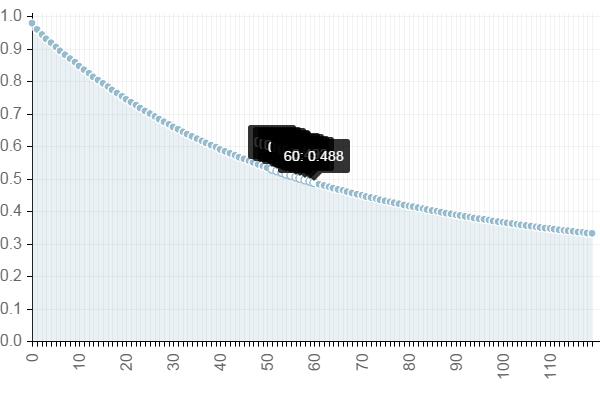
\includegraphics[scale=.5]{boston1940}
\caption{\label{fig:boston1940} Colon Cancer Survival Curve predicted from the data in 
Table~(\ref{tab:boston1940} using the neural network web app \url{http://ming-cancer.herokuapp.com/}.}
\end{figure}









Changing the data in Table~(\ref{tab:boston1940}) so that the address field is changed from Boston, Massachusetts to Denver, Colorado but keeping all other variables are unchanged results in the predicted probabilities of living at least 6, 12, and 60 months: .945, .902, .665. 
Behind the scenes, the apps use the input to the address field to make a call to the Google Maps API to convert the address into a latitude, longitude and elevation.
These probablities are noticeably higher and reflect both the documented effects of longitude and elevation on cancer treatment and prognosis in the United States.

An additional means of validating the predictions of these models is by comparing their predictions to each other for the same set of input data. IOBS is in the process of performing a systematic analysis of this type; all exploratory investigation to identify trends has shown the same effects for both the random forest and neural network versions of the models for each cacner type. For example, the effects of marital status and gender on survival prognosis in lung cancer (both men and women benefit from being married, but the effects are much more pronounced for men), are born out in both the random forest and neural network models. 

\section{Cancer and Proton/Photon Therapy}

The Lung, Breast, and Colon Cancer models described above take into consideration only variables that are known when a patient is first diagnosed. In constrast, the Prostate model also includes the SEER variable \codewhite{rx$\_$summ$\_$radiation}, which can take one one of the values:

\begin{itemize}[noitemsep]
\item Beam radiation
\item Combination of Beam and either implants or isotopes
\item None; diagnosed at autopsy
\item Patient or patient's guardian refused radiation therapy
\item Radioactive implants
\item Radiation, NOS - method or source not specified
\item Radioisotopes
\item Radiation recommended, unknown if administered
\item Unknown if radiation administered
\end{itemize}

As a first pass at investigating the effects of Radiation Therapy, especially Proton Therapy, one can compare different results of the model for different values of the above \codewhite{rx$\_$summ$\_$radiation} variable. For example, using the input data in Table \ref{tab:abq}, the model predicts a .52 probability of surviving 60 months. Changing the value of \codewhite{rx$\_$summ$\_$radiation} to \textbf{Beam radiation} results in a new predicted probability of surviving at least 60 months of .974.
Clearly, the effects of beam radiation are positive and large; the leap from observation to causality can be hazardous, however, if not analyzed correctly\footnote{``Simpson's Paradox,'' \url{http://www.intuitor.com/statistics/SimpsonsParadox.html}, accessed 11 Jan 2016.}. IOBS is looking into making these conclusions drawn from evidence-based, machine learning models more rigorous by firmly vetting them within the cutting-edge methods of Causality Calculus as pioneered by Judea Pearl.\footnote{Judea Pearl homepage at the University of California, Los Angeles, \url{http://bayes.cs.ucla.edu/jp_home.html}, accessed 11 Jan 2016.}





\begin{table}[tbp]
\begin{center}
\rowcolors{1}{white}{light-gray}
\begin{tabular}{lr}
  \toprule
  Variable  & Value \\ 
\midrule
  What is the tumor size (mm) & 40 \\  
  What is the patient's address? & Albuquerque new mexico \\ 
  Grade & moderately differentiated \\  
  Histology & adenomas and adenocarcinomas \\ 
  Laterality & not a paired site \\  
 Martial Status at Dx & Married including common law \\  
 Month of Diagnosis & Mar \\  
 How many primaries & 1 \\  
  Race$\_$ethnicity & White \\  
 rx$\_$summ$\_$radiation & Patient or patient's guardian refused radiation therapy \\
  seer$\_$historic$\_$stage$\_$a  & Localized/Regional \\ 
  Gender & Male \\  
  spanish$\_$hispanic$\_$origin & Non-spanish/Non-hispanic \\ 
 Year of Birth & 1960 \\  
  Year of Diagnosis & 2013 \\
\bottomrule
\end{tabular}
\caption{Example input data to the Prostate Cancer random forest Web app \url{http://prostate-cancer.herokuapp.com/}}
\label{tab:abq}
\end{center}
\end{table}


\appendix
\section{Pseudocode for the Data Transformation}
\label{subsec:pseudocode}

\begin{verbatim}
def train(X, T, D)
    // X, T, D are the original dataset
    X' = []
    D' = []

    // the transformation
    for each index i in X:
        for t=1 to T[i]:
            new_D = (0 if t < T[i], else D[i])
            append new_D to D'
            new_X = (X[i], t)
            append new_X to X'

    return a decision tree trained on (X', D')

def pmf(h, X)
    // X is a single datapoint
    // returns an array A where A[i] = P(Y = i | X)
    A = []
    p_so_far = 1 // this is p(T >= t | X)
    for t = 1 to (the last month where h has any data):
        // h knows p(T = t | T >= t, X), we call this p_cur
        p_cur = h's prediction for (X, t)
        append (p_so_far * p_cur) to A
        p_so_far *= (1 - p_cur)

\end{verbatim}


\bibliographystyle{plain}
%%\bibliographystyle{plainnat}
\bibliography{bobbib}
%\printbibliography{bobbib}
%\nocite{*}

\end{document}

